\documentclass[a4paper,10pt,fleqn]{article}

\usepackage{geometry}
\geometry{a4paper, top=25mm, left=35mm, right=30mm, bottom=30mm, headsep=10mm, footskip=12mm}
\usepackage{amsmath} 
\usepackage{amssymb}
\usepackage{amsthm} 
\usepackage{dsfont}
\usepackage{xcolor}
%\usepackage{enumerate}
%\usepackage{rotating}
\usepackage{cite}
\usepackage{pgfplots}
\usepackage[font=footnotesize,labelfont=bf,margin=12pt,format=hang]{caption}

\pgfplotsset{compat=newest}

\usetikzlibrary{arrows}
\usetikzlibrary{plotmarks}
\usepgfplotslibrary{groupplots}
%
%
%\newlength\figureheight
%\newlength\figurewidth
%
%
%\newcommand{\B}{\mathcal{B}} % box collection
%\newcommand{\Borel}{\mathfrak{B}} % Borel-\sigma-algebra
%\newcommand{\C}{\mathds{C}} % complex numbers
%\newcommand{\N}{\mathds{N}} % natural numbers
%\newcommand{\BigO}{\mathcal{O}} % big O notation
%\newcommand{\R}{\mathds{R}} % real numbers
%\newcommand{\Time}{\mathcal{T}} % time complexity
%\newcommand{\X}{\mathds{X}} % phase space
%\newcommand{\Z}{\mathds{Z}} % integer numerbs
%
%\newcommand{\algostep}[1]{{\tt {#1}:\newline}}
%\newcommand{\defword}[1]{\textbf{#1}}


%\definecolor{cpp_number}{RGB}{176,128,0}
%\definecolor{cpp_preprocessor}{RGB}{0,110,40}
%\definecolor{cpp_type}{RGB}{0,87,174}
%\definecolor{cpp_string}{RGB}{191,3,3}
%\definecolor{cpp_std}{RGB}{89,255,0}

\newcommand{\BTwelve}{\mathcal{B}_{12}}
\newcommand{\BTwelveVersion}[1]{\mathcal{B}_{12#1}}

\begin{document}



\section{Motivation} \label{sec:motivation}

This software is provided to analyse the dynamics of maps of the form
\begin{equation} \label{eq:map}
x_{n+1} = f \left( x_n \right)
\end{equation}
or flows given by an ODE
\begin{equation} \label{eq:flow}
\dot{x} \left( t \right) = f \left( t, x \left( t \right) \right), \quad t \in \left[ t_0, t_{end} \right]
\end{equation}
using a set-oriented ansatz. It relies on the idea of the software package GAIO, see \cite{dellnitz2001algorithms}, but utilises massive parallelisation on both CPU and graphics cards (GPU).\\
Based on a surrounding hyperrectangle/box, one can gradually bisect boxes in arbitrary coordinate direction, discard them or insert new boxes. For a three-dimensional illustrative example, see figure \ref{fig:box_tree}. In addition, one can set flags in each box, see also section \ref{subsec:integer_data_types}. While in GAIO the whole tree is stored, here only the leaves are explicitly stored. It means in effect that by setting a flag of a box in smaller depth, all its descendants inherit this flag automatically. Vice versa, a flag in such a box is seen as set if and only if all of its descendant leaves have the flag set. Apart from that, all ``tree algorithms'' are supposed to yield the same results in both software packages.\\
Here, so called point iterators are additionally provided. As example, see figure \ref{fig:point_iterator}. There, four two-dimensional boxes are displayed. The point iterator traverses each box and therein an inner grid with $4^2$ points. Each grid point can be mapped with an arbitrary map; in figure \ref{fig:point_iterator}, the identity map is used. The numbers indicate the order of traversing. Yet, those points are not stored explicitly. That means, they are only computed when needed. This saves memory and increases memory bandwidth.
\begin{figure}
	\centering
	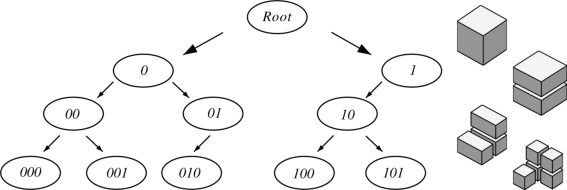
\includegraphics[width=0.75\linewidth]{pics/box_tree.pdf}
	\caption[Hierarchical storage of the box collections in the software package GAIO]{Hierarchical storage of the box collections in the software package GAIO. Illustration taken from \cite{dellnitz2002set}.}
	\label{fig:box_tree}
\end{figure}
\begin{figure}
	\centering
	{\tiny
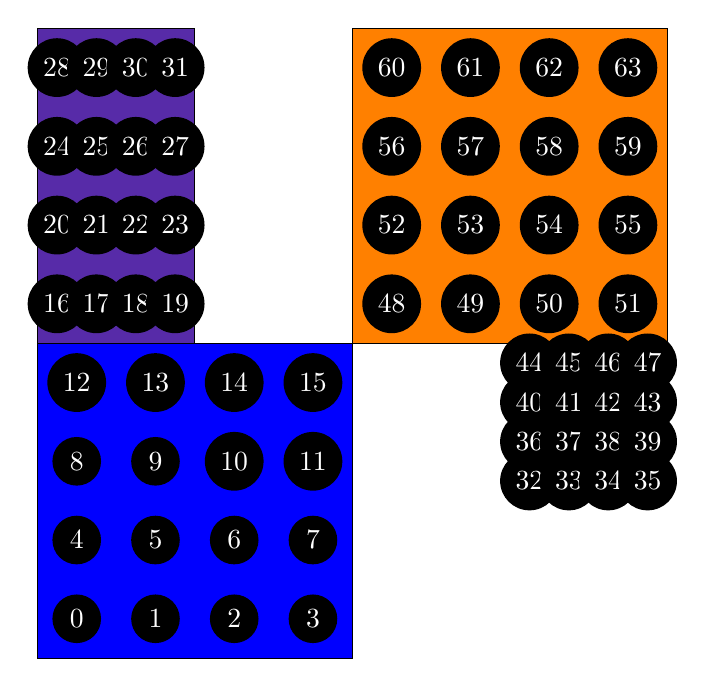
\begin{tikzpicture}
  \newcounter{grid}
  \setcounter{grid}{0}
  
  \draw[fill=blue] (0.5,0.5) rectangle (4.5,4.5) {};
  \draw[fill=blue!66!orange] (0.5,4.5) rectangle (2.5,8.5) {};
  \draw[fill=blue!33!orange] (6.5,2.5) rectangle (8.5,4.5) {};
  \draw[fill=orange] (4.5,4.5) rectangle (8.5,8.5) {};
  
  \foreach \y in {1,2,3,4} {
    \foreach \x in {1,2,3,4} {
      \node at (\x,\y) [circle,white,fill=black] { \thegrid };
      \addtocounter{grid}{1}
    }
  }
  
  \foreach \y in {5,6,7,8} {
    \foreach \x in {0.75,1.25,1.75,2.25} {
      \node at (\x,\y) [circle,white,fill=black] { \thegrid };
      \addtocounter{grid}{1}
    }
  }
  
  \foreach \y in {2.75,3.25,3.75,4.25} {
    \foreach \x in {6.75,7.25,7.75,8.25} {
      \node at (\x,\y) [circle,white,fill=black] { \thegrid };
      \addtocounter{grid}{1}
    }
  }
  
  \foreach \y in {5,6,7,8} {
    \foreach \x in {5,6,7,8} {
      \node at (\x,\y) [circle,white,fill=black] { \thegrid };
      \addtocounter{grid}{1}
    }
  }
\end{tikzpicture}
}
	\caption[Illustration of point iterators]{Illustration of point iterators. Each black circle indicates a grid point, which is mapped with the identity map. The numbers inside indicate the ordering, i.e. the ``begin'' iterator points to 0 and the ``end'' iterator points to (imaginary) 64.}
	\label{fig:point_iterator}
\end{figure}



\section{Installation} \label{sec:installation}

\subsection{Version Management} \label{subsec:version_management}

Different versions of $\BTwelve$ are treated with lower case letters starting from \verb$a$, i.e. $\BTwelveVersion{a}$, $\BTwelveVersion{b}$, and so on. In the following, the versions are denoted by $\BTwelveVersion{x}$ or \verb$B12x$.

\subsection{Requirements} \label{subsec:requirements}

Using this software requires the following packages:
\begin{itemize}
\item CUDA, at least version 7.0, and its requirements.
\end{itemize}
If one additionally wants to use the Matlab interface, one needs
\begin{itemize}
\item Matlab, at least version R2013b (8.2), and
\item Boost, at least version 1.31.
\end{itemize}
It is also recommended to install
\begin{itemize}
\item OpenMP,
\item a CUDA-capable GPU with compute capability $\geq 2.0$, and
\item CMake, at least version 3.5.
\end{itemize}


\subsection{Definition of Custom Maps} \label{subsec:def_custom_maps}

To use $f$ of \eqref{eq:map} or \eqref{eq:flow} a C++ functor needs to be implemented, i.e. a class/struct with member function \verb$operator()$. In the following, we want to implement $f$ of \eqref{eq:map} or \eqref{eq:flow} calling the corresponding functor \verb$MyMap$.\\
First, create the header file \verb$B12x/src/include/Map_MyMap.h$. This header file must
\begin{itemize}
\item be guarded against redefinition via preprocessor directives,
\item include \verb$MapTools.h$,
\item define the functor \verb$MyMap$
	\begin{itemize}
	\item that is included in the \verb$b12$ namespace,
	\item that inherits from \verb$public thrust::binary_function<REAL*,REAL*,bool>$ where \verb$REAL$ stands for the floating point type,
	\item whose member functions are all inlined and declared as both host and device function,
	\item whose constant \verb$operator()$ member function additionally takes a constant real pointer as input and a non-constant real pointer as output and returns a boolean, and
	\item that is (only) templated by Dimension and floating point type if you want to use CMake compilation or the Matlab interface.
	\end{itemize}
\end{itemize}
That is, the minimal source code defining the functor \verb$MyMap$ might look like this:
\begin{verbatim}
#pragma once

#include "MapTools.h"

namespace b12 {

template<Dimension DIM, typename REAL>
struct MyMap : public thrust::binary_function<REAL*, REAL*, bool>
{
  __host__ __device__
  inline bool operator()(const REAL *, REAL *) const;
};

} // namespace b12
\end{verbatim}
For a more general approach, consider implementing a help functor defining the right-hand side of \eqref{eq:map} or \eqref{eq:flow}. This functor can then be wrapped into the actual functor \verb$MyMap$ by using \verb$IteratingMap$ for \eqref{eq:map} to allow the use of function composition, i.e. $f^k$ for any $k = 0, 1, 2, \ldots, 2^{32}-1$, or \verb$RK4$ for \eqref{eq:flow} to solve the non-autonomous ODE (or \verb$RK4Auto$ when autonomous) by means of the classical Runge-Kutta method where the step size and step number can be set. For this, also see \verb$Map_Henon.h$ and \verb$Map_Lorenz.h$.\\
To obtain maximal efficiency, the functor should
\begin{itemize}
\item use static, i.e. known at compile time, indices for the pointers given as arguments in \verb$operator()$, which can also be realised by unrolled loops, see e.g.\\ \verb$Map_Identity.h$,
\item not allocate dynamic memory,
\item be implemented separately for single and double precision if the right-hand side of \eqref{eq:map} or \eqref{eq:flow} contains functions for which the CUDA compiler provides different floating-point versions, e.g. for trigonometric, logarithmic, exponential or probabilistic functions, also see \verb$Map_Standard.h$.
\end{itemize}


\subsection{Compilation} \label{subsec:compilation}

Copy the $\BTwelveVersion{x}$ folder into a location with enough available memory space, usually of the order of double-digit gigabytes depending on the amount of desired combinations of architectures, compute capabilities, phase space dimensions, floating-point types, and so on, see section~\ref{subsubsec:cmake_compilation} for more details.\\
%After compilation is finished, make sure that all directories and files can be read and executed, e.g. via the command \verb$chmod -R a+rx /opt/B12$.\\
Note that compilations may occupy extremely much time, especially for GPU code!

\subsubsection{Plain Compilation} \label{subsubsec:plain_compilation}

When neither CMake nor the Matlab interface is required, one may compile its \verb$.cu$ files with the nvcc compiler using the following flags:
\begin{itemize}
\item[] \verb$-arch=sm_**$ \; to generate code for the correspondig GPU / compute capability,
\item[] \verb$-std=c++11$ \; to enable C++11 support,
\item[] \verb$-O3$ \; to let the compiler optimise the code, and
\item[] \verb$-Xcompiler -fopenmp -lgomp$ \; to allow OpenMP parallelization on CPU.
\end{itemize}

\subsubsection{CMake Compilation} \label{subsubsec:cmake_compilation}

This is the recommended way for compiling. When a source code modification is implemented, e.g. the creation of a new map functor, only the dependent files are automatically (re)compiled.\\
To use this method, one should modify \verb$B12x/UserSettings.txt$ containing the following variables:
\begin{itemize}
\item[] \verb$computeCapability$ \; \ldots the compute capability for which the code is compiled for (when no GPU is available, use a value like 3.5),
\item[] \verb$installPath$ \; \ldots the installation directory, i.e. \verb$installPath/B12/B12x$ will contain the compiled library,
\item[] \verb$ThrustArchitectures$ \; \ldots list of memory/parallelisation schemes (\verb$CPP$: sequential on CPU, \verb$OMP$: parallel on CPU using OpenMP, \verb$CUDA$: parallel on GPU),
\item[] \verb$Dimensions$ \; \ldots list of phase space dimensions,
\item[] \verb$Reals$ \; \ldots list of C++ floating-point types (only \verb$float$ and \verb$double$ supported),
\item[] \verb$MaxDepths$ \; \ldots list of maximal depths for the \verb$ImplicitBoxTree$, also see section \ref{sec:usage},
\item[] \verb$Grids$ \; \ldots list of grid functors (currently only \verb$InnerGrid$ and \verb$FullGrid$ are tested),
\item[] \verb$Maps$ \; \ldots list of map functors, which also implicitly contains the identity map for all dimensions defined in \verb$Dimensions$.
\end{itemize}
To include \verb$MyMap$, one should define a variable with this name as list of two strings consisting of integers, e.g. \verb$set(MyMap "2 3" "3 5")$. In this example, \verb$MyMap$ would be compiled for the dimensions 2 and 3 where the constructors take 3 and 5 arguments, respectively. Subsequently, add \verb$"MyMap"$ to the list \verb$Maps$.\\
Afterwards the libraries can be compiled and built with CMake. For Linux systems e.g., open a terminal and type in the following commands:
\begin{verbatim}
cd [path to the B12x folder]/build
cmake ..
make -j4
make -j4
make -j4
sudo make install
sudo make install
\end{verbatim}
The number behind the \verb$j$ indicates the number of cores used to parallelise compilation.\\
Afterwards, make sure that the software package can be found by using the command:
\begin{verbatim}
echo 'export PATH=/opt/B12/B12x/:${PATH}' >> ~/.bashrc
\end{verbatim}


\subsection{Uninstallation} \label{subsec:uninstallation}

To uninstall $\BTwelveVersion{x}$, only the folders \verb$B12x$ containing the software need to be deleted.



\section{Usage} \label{sec:usage}

\subsection{Integer Data Types} \label{subsec:integer_data_types}

Even though in Matlab 64 bit integers are used to represent count numbers and indices, always pay attention to the underlying data types, especially to their ranges.

\subsubsection*{Dimension ($0, \ldots, 255$)}

stands for possible phase space dimensions for \eqref{eq:map} and \eqref{eq:flow}.

\subsubsection*{Depth ($0, \ldots, 255$)}

indicates the actual depth in ImplicitBoxTrees. In particular, 0 stands for the tree's root, \verb$getLeafDepth()$ = 255 = -1 for its leaves, and \verb$getUnsubdividableDepth()$ = 254 = -2 for nodes that are not leaves and whose only child is a leaf or both children are leaves. The maximal possible depth is determined by the template parameter, see section \ref{subsec:cpp}, but not greater than 253.

\subsubsection*{NrBoxes ($0, \ldots, 2^{32}-1 = 4,294,967,295)$}

is basically used indicating search indices or box counts. The largest value, also representable as \verb$NrBoxes(-1)$, is reserved for the search index ``not found''.

\subsubsection*{NrPoints ($0, \ldots, 2^{64}-1)$}

is internally used to index points. Therefore, using at least $2^{64}$ points at once leads to undefined behaviour.

\subsubsection*{Flags}

ranges actually form $0$ to $255$. But it should actually be seen as a type storing eight different on/off states, representable as powers of two. That is, $4$ e.g. stands for the third state, while $73 = 64 + 8 + 1$ stands for the seventh, fourth, and first state. The meaning of each state is up to the user's decision. Besides, there is the enumeration declaration \verb$Flag$ containing \verb$NONE$ = 0, \verb$HIT$ = 1, \verb$INS$ = 2, \verb$EXPD$ = 4, \verb$SD$ = 8, \verb$EQU$ = 16, \verb$ENTR$ = 32, \verb$EXTR$ = 64, and \verb$ALL$ = 255. By design, checking whether the Flag \verb$NONE$ = 0 is set always yields true.


\subsection{C++} \label{subsec:cpp}

When implementing plain CUDA C++ code, include \verb$Grids.h$, the relevant \verb$Map_MyMap.h$, and \verb$ImplicitBoxTree.h$. Unless the corresponding libraries are already precompiled and installed, define the preprocessor variable \verb$INCLUDE_IMPLICIT_BOX_TREE_MEMBER_DEFINITIONS$ before including. The header files can be found in \verb$B12x/src/include$.\\
The class \verb$ImplicitBoxTree$ is templated by the enumeration declaration \verb$Architecture$, see section \ref{subsubsec:cmake_compilation}, \verb$Dimension$ for the desired phase space dimension of \eqref{eq:map} and \eqref{eq:flow}, a floating-point precision (default = double) for the coordinate computations, and an unsigned 8-bit integer (default = 64) representing the maximal possible depth, which can take on the values 32, 64, 72, 80, 96, and 128. For example, \verb$ImplicitBoxTree<CUDA, 3, float, 96>$ is a valid type. All the member methods are described in \verb$ImplicitBoxTree.h$. The same applies for \verb$Grids.h$.\\
As simplification to distinguish between CPU and GPU, see the implementations in\\ \verb$ThrustSystem.h$. In particular, \verb$ThrustSystem<A>::Vector<T>$ can be used as vector storage type, where \verb$A$ stands for an \verb$Architecture$ and \verb$T$ for an arbitrary type,\\
\verb$typename ThrustSystem<A>::execution_policy()$ as parallelisation scheme for Thrust algorithms, and \verb$ThrustSystem<A>::Memory::isOnHost()$ as boolean indicating which memory is used.

\subsubsection*{Example for 20 iterations of the subdivision algorithm with the H\'{e}non map}

\begin{verbatim}
#include "Grids.h" 
#include "Map_Henon.h"
#define INCLUDE_IMPLICIT_BOX_TREE_MEMBER_DEFINITIONS
#include "ImplicitBoxTree.h"
#undef INCLUDE_IMPLICIT_BOX_TREE_MEMBER_DEFINITIONS

using namespace b12;

int main()
{
  const Architecture A = CUDA;
  const Dimension DIM = 2;
  
  ThrustSystem<A>::Vector<double> center(DIM, 0.0);
  ThrustSystem<A>::Vector<double> radius(DIM, 3.0);
  
  // create tree with surrounding box: [-3, 3]^2
  ImplicitBoxTree<A, DIM, double, 64> ibt(center, radius);
  
  // create an inner grid scheme with 10^DIM points for each box
  InnerGrid<DIM, double> grid(10);
  
  // create Henon map functor with parameters 1.4 and 0.3, once applied
  Henon<DIM, double> map(1.4, 0.3, 1);
  
  // set the Flag SD in the root
  // child nodes/boxes inherit the Flags while subdividing
  ibt.setFlags(Flag::SD, 0);
  
  for (int i = 1; i <= 20; ++i) {
    // subdivide all leaf boxes that have Flag SD set
    ibt.subdivide(Flag::SD);
    
    // define a iterator pair representing the range, i.e. [begin, end),
    // of all points created by grid for each leaf box and mapped by map;
    // NOTE: After the ImplicitBoxTree has changed, such an iterator has
    // undefined behaviour!!!
    auto itPair = ibt.makePointIteratorPairOverLeaves(grid, map);
    
    // set the Flag HIT in all leaf boxes that are 'hit' by the mapped points
    ibt.setFlagsByIterators(itPair, Flag::HIT, -1);
    
    // remove all leaf boxes (and corresponding parents) that have HIT not set
    ibt.remove(Flag::HIT);
    
    // unset HIT for next iteration
    ibt.unsetFlags(Flag::HIT, -1);
    
    // print iteration and number of leaves
    std::cout << i << ": " << ibt.count(-1) << std::endl;
  }
  
  return 0;
}
\end{verbatim}


\subsection{Matlab}

To use $\BTwelveVersion{x}$ in Matlab, one should add the appropriate folder to Matlab's search path by calling \verb$addpath(genpath('/opt/B12/B12x/matlab'));$\\
After installation, the following classes are provided. Their instructions can be found in the corresponding m-files stored in \verb$/opt/B12/B12x/matlab$.

\subsubsection*{ImplicitBoxTree, ompImplicitBoxTree, gpuImplicitBoxTree}

All three classes represent the ImplicitBoxTree class, where ImplicitBoxTree works sequentially on CPU, ompImplicitBoxTree in parallel (OpenMP) on CPU, and gpuImplicitBoxTree on GPU. The ``template arguments'', see section \ref{subsec:cpp}, are passed via a cell array into the constructor. Note that the assignment operator only works as shallow copy. For a deep copy, use the (copy) constructor. It is also worth mentioning that many member functions have only one version, whose behaviour depends on the input, see e.g. \verb$setFlags$, compared to their C++ code equivalents, e.g. \verb$setFlags$, \verb$setFlagsByIterators$, \verb$setFlagsByPoints$, \verb$setFlagsBySearch$, and \verb$setFlagsByStencil$. That is why there are no methods like \verb$makePointIteratorPair$.

\subsubsection*{GridFunctor, MapFunctor}

Both classes have the same structure. The first component is the string indicating the C++ type, i.e. for GridFunctor ``InnerGrid'' or ``FullGrid'' and for MapFunctor ``MyMap'' are valid. The second component stores the dimension while the third one stores the vector of constructor arguments.

\subsubsection*{Example programs}

In \verb$B12x/matlab$, you can find some example implementations to become more familiar with the usage in Matlab.

\subsubsection*{Equivalent example from above}

\begin{verbatim}
addpath(genpath('/opt/B12/B12x/matlab'));

DIM = 2; HIT = 1; SD = 8;

% create tree on GPU with surrounding box: [-3, 3]^2
ibt = gpuImplicitBoxTree([0;0], [3;3], {DIM, 'double', 64});

% create an inner grid scheme with 10^DIM points for each box
G = GridFunctor('InnerGrid', DIM, 10);

% create Henon map functor with parameters 1.4 and 0.3, once applied
M = MapFunctor('Henon', DIM, [1.4, 0.3, 1]);

% set the Flag SD in the root
% child nodes/boxes inherit the Flags while subdividing
ibt.setFlags('all', SD);

for i = 1:20
    % subdivide all leaf boxes that have Flag SD set
    ibt.subdivide(SD);
    
    % a cell array containing a grid, a map, a depth, and a Flag;
    % in each leaf box (depth = -1) that have Flags 0 set, i.e. in effect
    % all boxes, 10^2 inner grid points are created and then mapped via
    % the Henon map
    scheme = {G, M, -1, 0};
    
    % set the Flag HIT in all leaf boxes that are 'hit' by the mapped points
    ibt.setFlags(scheme, HIT, -1);
    
    % remove all leaf boxes (and corresponding parents) that have HIT not set
    ibt.remove(HIT);
    
    % unset HIT for next iteration
    ibt.unsetFlags('all', HIT);
    
    % print iteration and number of leaves
    fprintf('%2d: %9d\n', ibt.depth(), ibt.count(-1));
end
\end{verbatim}





\bibliography{papers.bib}
\bibliographystyle{plain}


\end{document}
